\clearpage

\section{\label{systematic}Systematic Uncertainties}
% The systematic uncertainties were studied for the spectra and $R_{\rm CP}$ analysis. Several sources are contributed to the uncertainties. Such as the TPC tracking, the raw yield extraction, the daughter $p_T$ cut scan, the topological cuts scan, the double counting and the vertex resolution contribution and so on. 
%
% The TPC uncertainties were studied by comparison of the tracking performance from real data and the MC simulation. A few different methods were used to extract the raw $D^0$ signal counts, for example using the like-sign method or mixed-event technique to subtract the combinatorial background, or using the binning counting method instead of directly fitting method to extract the yield. Several different daughter $p_T$ cuts were applied on the $D^0$ reconstruction and corrected for the efficiency. We also varied the topological variables for the reconstruction with a quite different reconstruction efficiency. The mis-identification from the daughter particles were studied. The vertex resolution was also discussed in the previous section.
%

The approach for the $D^0$ spectrum systematic uncertainties are well studied. Several sources can be contributed to the uncertainties. The first one is coming from the raw yield extraction. We varied the signals extraction methods instead of use binning counting methods, we tried using fitting method, tried vary the fitting range, and also tried using likesign for background to estimate the uncertainties for raw yield extraction. 

The second source would be coming from the TPC embedding uncertainties, this one is well studied by comparison the nHits and Dca distributions between data and embedding. Here the real data iswithout HFT in tracking. This is a self-produced testing sample with the office library and chain option. Fig.~\ref{nHits_0_80} and Fig.~\ref{Dca_0_80} show the nHits and Dca comparison between real data and embedding for 0-80\% centrality. Bottom panels show the double ratio, and a fitted line as guidance. As seen, the embedding sample can reproduce the real data reasonable well. Then the systematic uncertainties can be estimate by varying the cuts from nHits$>$20 to nHits$>$25, and Dca$>$1.0 to Dca$>$1.5 as Equ.~\ref{nHitDca_eq}. 

\begin{equation}
  \begin{aligned}
  r_{nHits} = (nHits>25)/(nHits>20)_{data} / (nHits>25)/(nHits>20)_{MC} \\
  r_{Dca} = (Dca>1.5)/(Dca>1.0)_{data} / (Dca>1.5)/(Dca>1.0)_{MC}
\end{aligned}
\label{nHitDca_eq}
\end{equation}

Then after varying nHits and Dca, the comparison of data and embedding shown as Fig.~\ref{nFit_Dca_Ratio_7} for nHits (left) and Dca (right). The bottom panels show these double ratio, and quote as systematic uncertainties. For the $R_{CP}$ calculations, at some point they are correlated for central and peripheral collisions and somehow can be canceled out. So, for the $R_{CP}$ systematic, we using $r_{nHits}-cent / r_{nHits}-peripheral$ to calculate the uncertainties. The nHits, Dca and TofPID (as discussed in the pid part) systematic are added up quadratical for single track. For the $D^0$ calculations, the pion and kaon tracks are added linearly.

\begin{figure}[htbp]
\begin{minipage}[htbp]{0.45\linewidth}
\centering
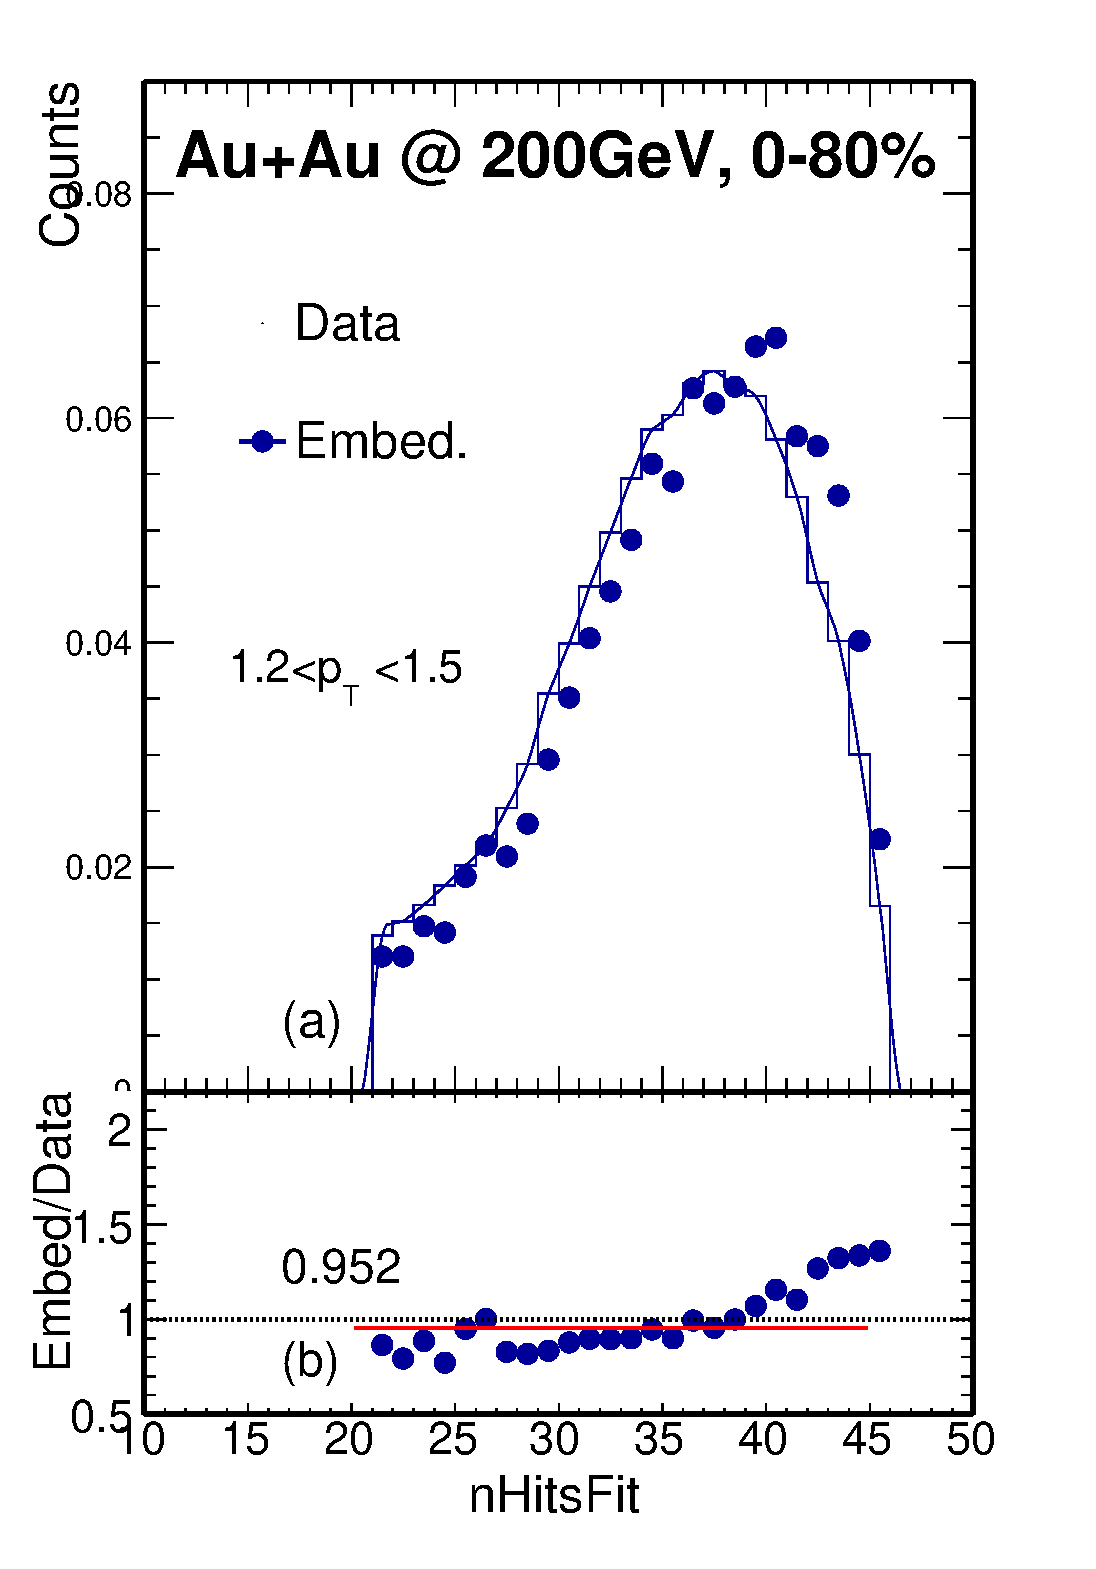
\includegraphics[width=1.0\textwidth,angle=0]{figure/Run14_D0HFT/nHitsFit11_6.eps}
\caption{ nHits comparison between real data and embedding for 0-80\%. \label{nHits_0_80}}
\end{minipage}
\hfill
\begin{minipage}[htbp]{0.45\linewidth}
\centering
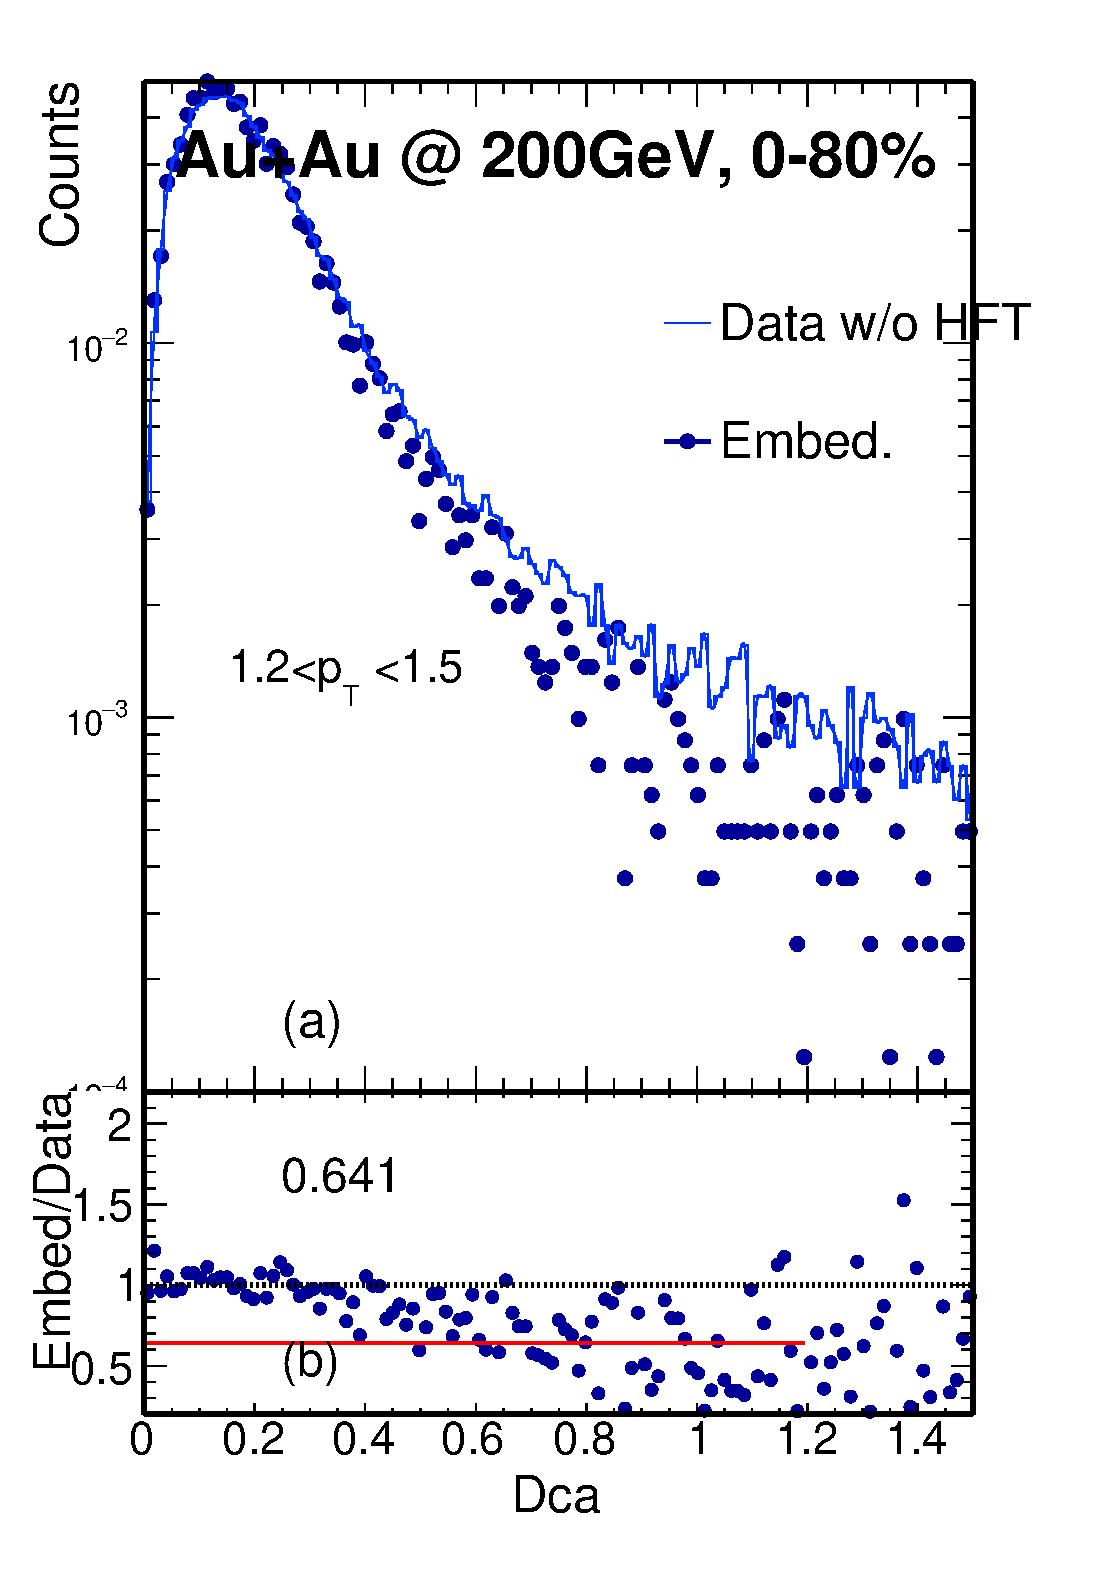
\includegraphics[width=1.0\textwidth,angle=0]{figure/Run14_D0HFT/Dca11_6.eps} 
\caption{ Dca comparison between real data and embedding for 0-80\%. \label{Dca_0_80}}
\end{minipage}
\end{figure}

\begin{figure}[htbp]
\centering
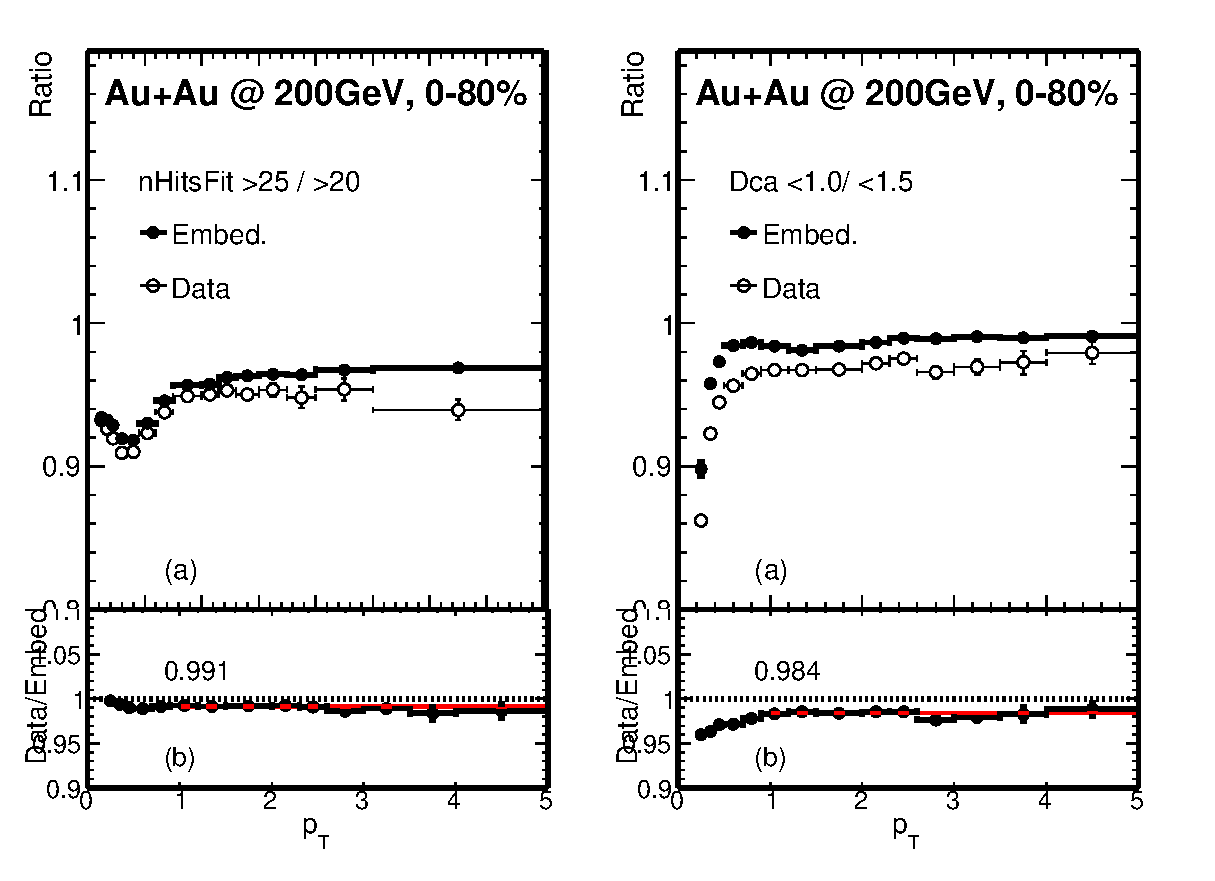
\includegraphics[keepaspectratio,width=0.9\textwidth]{figure/Run14_D0HFT/nFit_Dca_Ratio_7.eps}
\caption{Varying nHit(left) and Dca(right) comparison between real data and embedding for 0-80\% }
\label{fig:nFit_Dca_Ratio_7}
\end{figure}

%The next one is from the fast-simulation part, as discussed in the previous section, there are $\sim$5\% difference between the pure Hijing and fast-simulation relay on Hijing when we validating the packages. We quote this 5\% contribution as one of the systematic sources.
%Another source would be the vertex resolution contribution as we discussed before, since the most central collisions does not suffer the vertex contribution while the impact on the most peripheral collisions could be visible. We quote a separate systematic errors for difference centralities, 10\% for the most peripheral (40-80\%) collision, 5\% for the mid-central collisions (10-40\%) and 0 for the most central (0-10\%) collisions. 
%The next one source coming from the bin shift correction, there are several functions can be used for the bin correction such as the levy function and fonll function, the difference between these two methods are quoted as one of the systematic source. 

The next source is by varying the topological cuts and daughter $p_t$ cuts. The standard TMVA cuts, the 50\% efficiency and 150\% efficiency cuts are calculated, and also the daughter $p_T$ cuts are checked for 300 MeV and 500 MeV beside of the default value 600 MeV. The difference between the corrected yield are quoted as the systematic source. Also there is a source coming from the double counting and vertex resolution contribution as we discussed in the previous sections.

Note here, for the $R_{CP}$ calculations since there are correlated uncertainties, so similar as TPC part,for the daughter $p_T$ scan and topological cuts scan uncertainties, we calculate the $R_{CP}$ for each individual setup or cuts, then quota the difference of $R_{CP}$ for each cuts as systematic errors. For the others, such as yield extraction, double counting and vertex resolutions, those uncertainties was quadratical added up for $R_{CP}$.

Fig.~\ref{sysErr_0_10} to Fig.~\ref{sysErr_0_80} shows the $D^0$ spectrum different sources contribution in various centralities. As we see, the systematic uncertainties is quite small in the most of the $p_T$ range except some of the $p_T$ ranges due to the limited statistics and large contribution from yield extraction.

\begin{figure}[htbp]
\begin{minipage}[htbp]{0.47\linewidth}
\centering
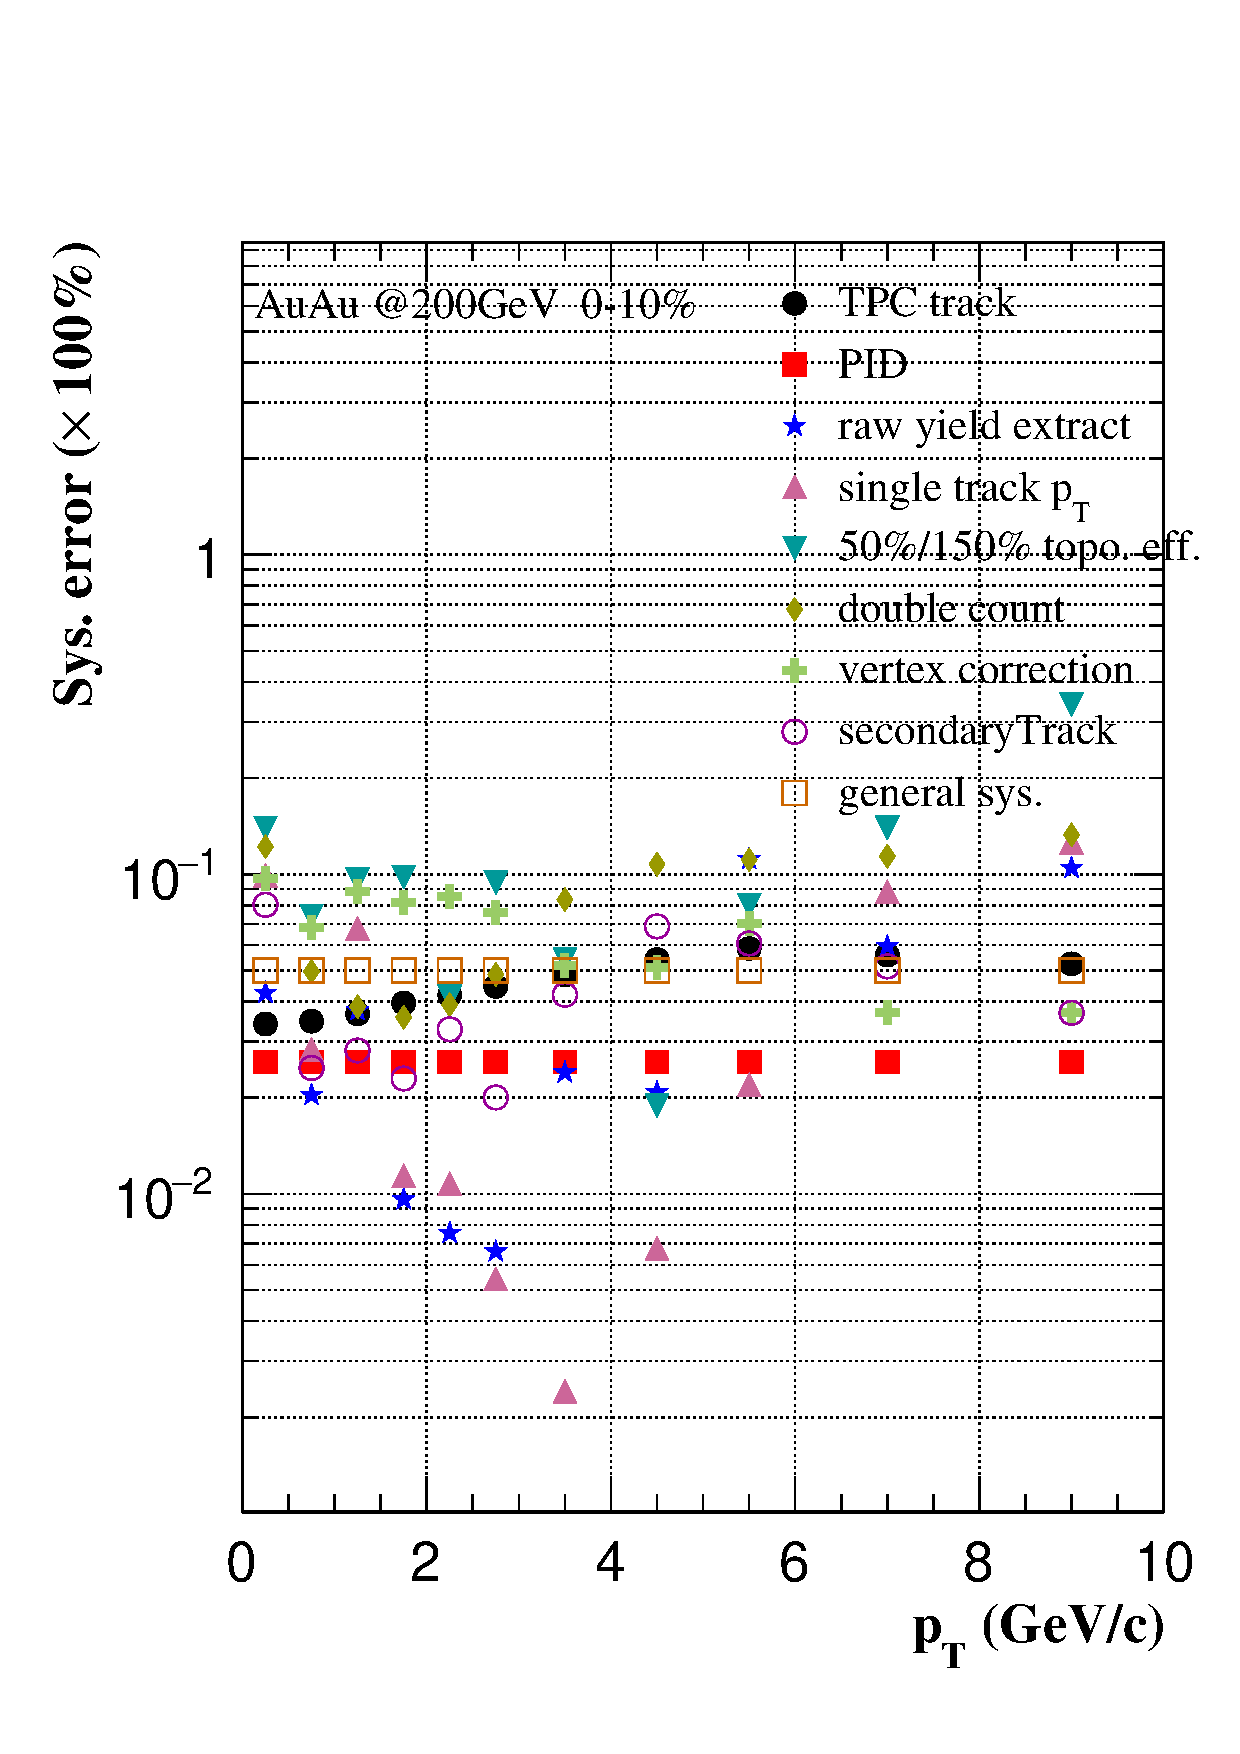
\includegraphics[width=1.0\textwidth,angle=0]{figure/Run14_D0HFT/sysErr_0_10_2.pdf}
\caption{ Systematic uncertainties from different sources for 0-10\% spectra. \label{sysErr_0_10}}
\end{minipage}
\hfill
\begin{minipage}[htbp]{0.47\linewidth}
\centering
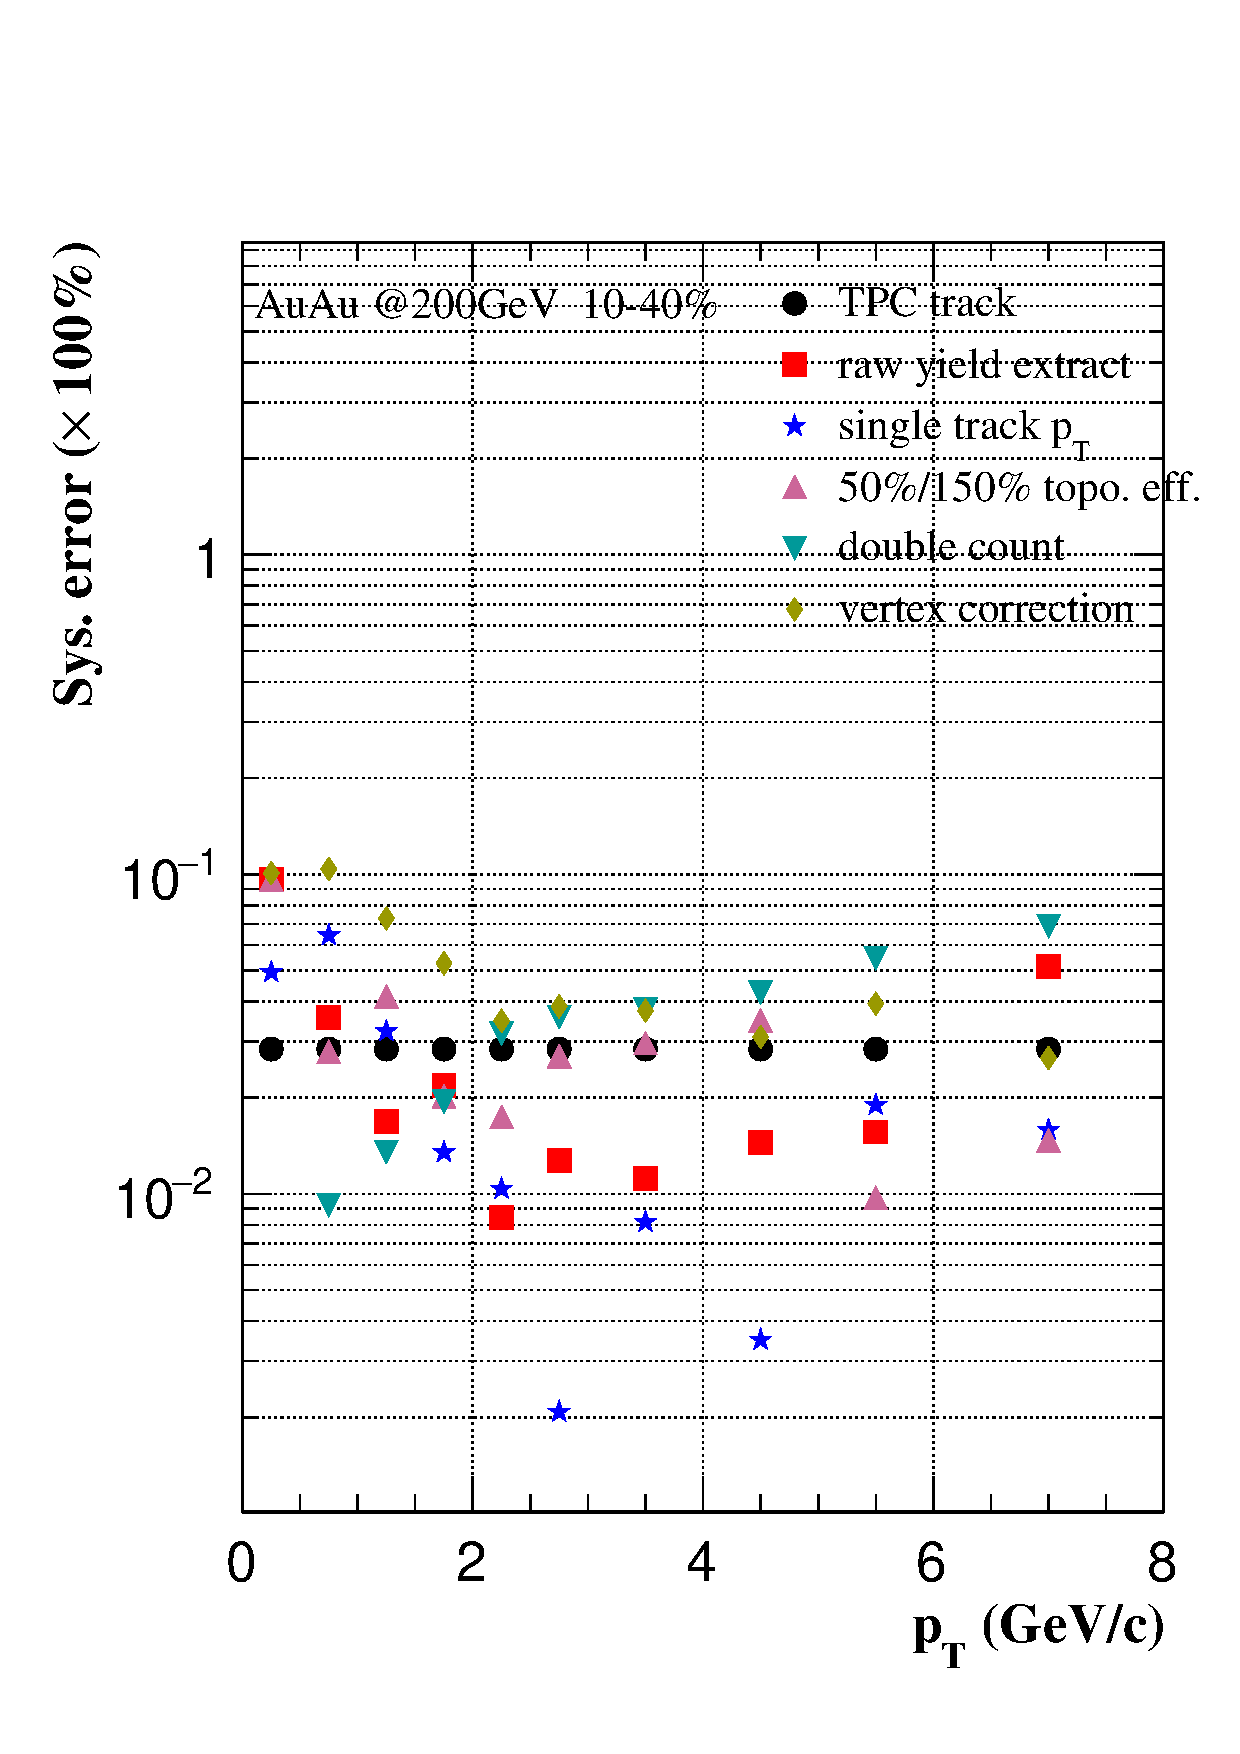
\includegraphics[width=1.0\textwidth,angle=0]{figure/Run14_D0HFT/sysErr_10_40_2.pdf} 
\caption{ Systematic uncertainties from different sources for 10-40\% spectra. \label{sysErr_10_40}}
\end{minipage}
\end{figure}

\begin{figure}[htbp]
\begin{minipage}[htbp]{0.47\linewidth}
\centering
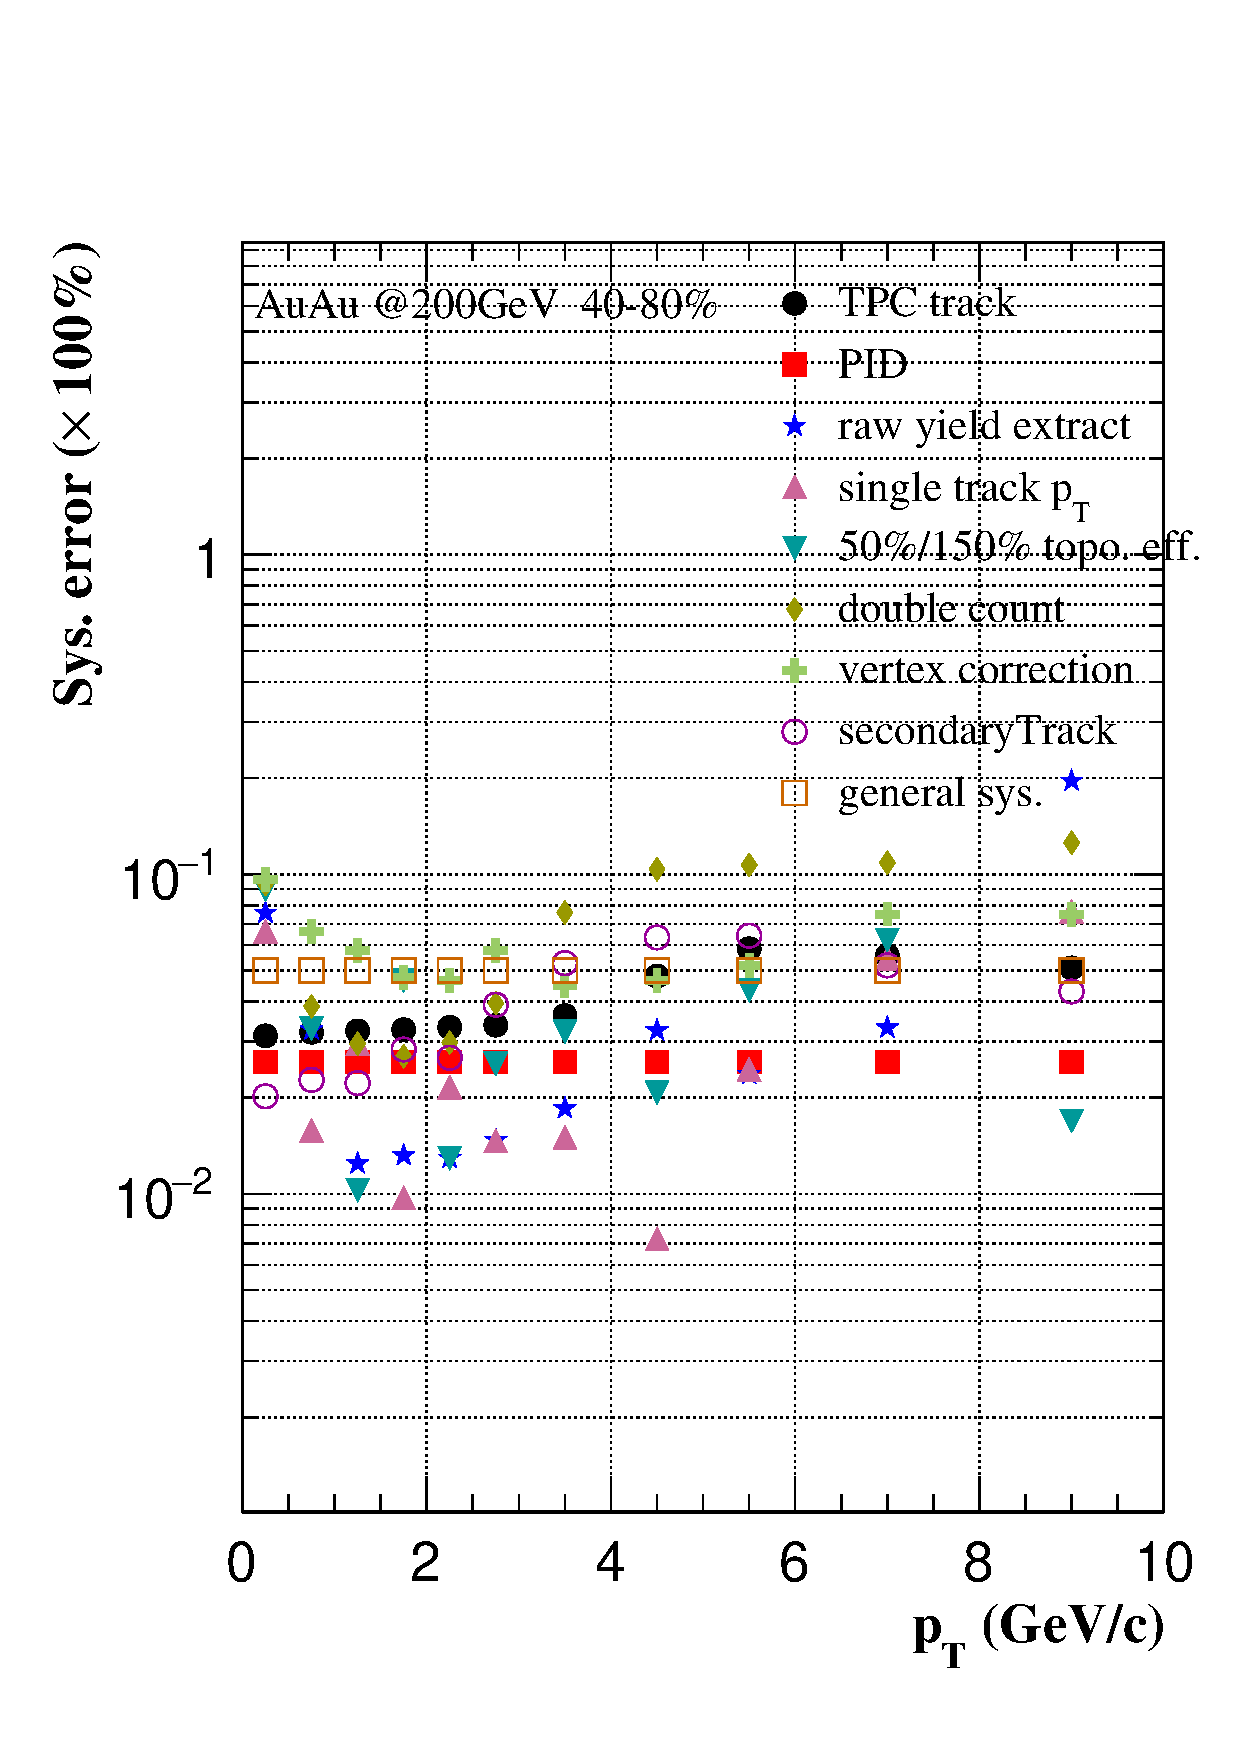
\includegraphics[width=1.0\textwidth,angle=0]{figure/Run14_D0HFT/sysErr_40_80_2.pdf}
\caption{ Systematic uncertainties from different sources for 40-80\% spectra. \label{sysErr_40_80}}
\end{minipage}
\hfill
\begin{minipage}[htbp]{0.47\linewidth}
\centering
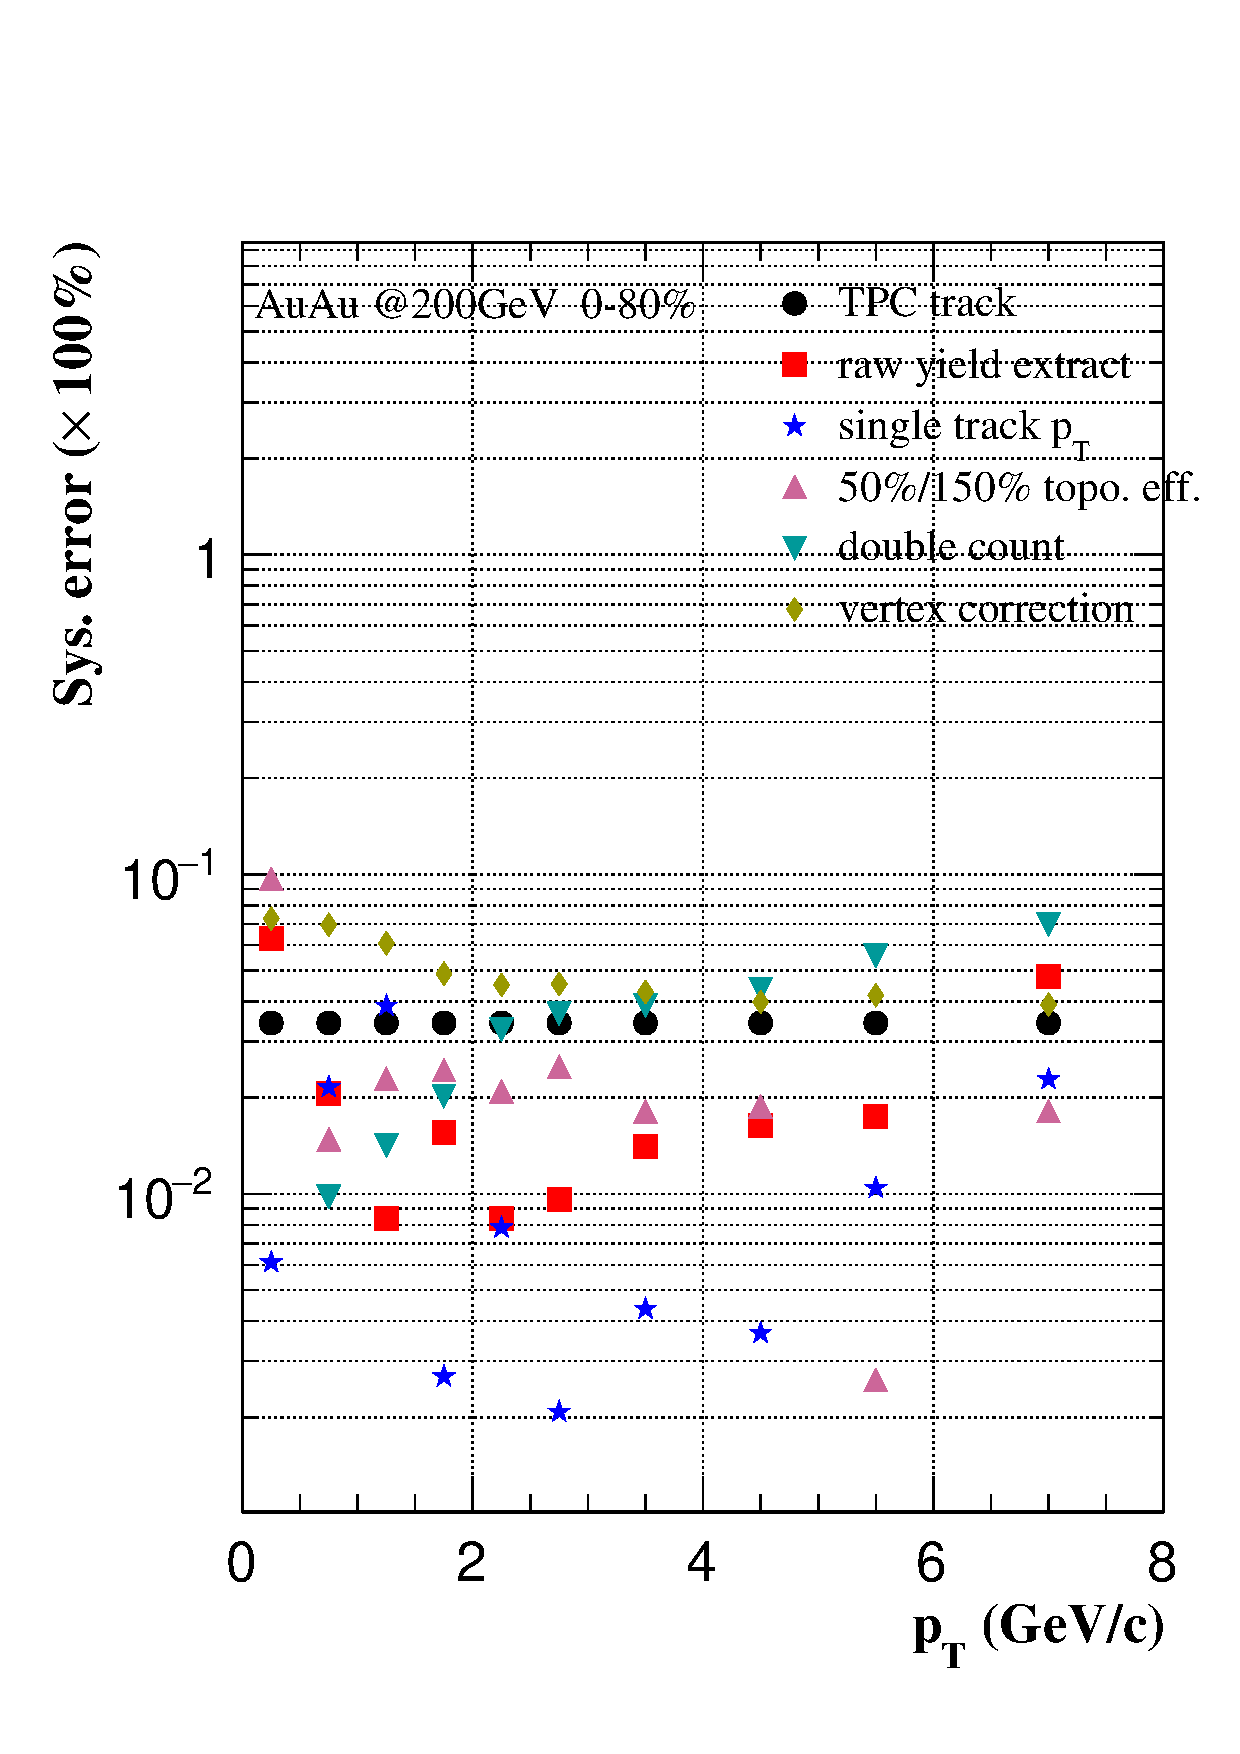
\includegraphics[width=1.0\textwidth,angle=0]{figure/Run14_D0HFT/sysErr_0_80_2.pdf} 
\caption{ Systematic uncertainties from different sources for 0-80\% spectra. \label{sysErr_0_80}}
\end{minipage}
\end{figure}


% For the $R_{AA}$ results shown later, they share the most of the systematic uncertainties with the spectrum, but for the TPC part, the TPC contribution from Au+Au and p+p collisions can be canceled out. The black bracket only represented the uncertainties from Au+Au.

% \begin{table}[htp]
% \centering
% \caption{Systematic uncertainties from different sources}
% \label{syserr}
% 	\begin{center}
% 	\begin{tabular}{l|l|l|l|l|l|l|l}
%   \Xhline{1.6pt}
%   $p_T$ range&Yield extra&Embedding&fast-simu&Topo Scan&bin shift&daughter $p_T$&total\\ \hline
%   0.0 -  0.5  &   0.28575        &  0.06     &  0.05           & 0.150186  &  0.206038   &  0.0961785  &   0.402506  \\ \hline
% 	0.5 - 1.0   &   0.276043       &  0.06     &  0.05           & 0.124592  &  0.0641394  &  0.104796   &   0.336034  \\ \hline
% 	1.0 - 1.5   &   0.0332581      &  0.06     &  0.05           & 0.08445   &  0.0416632  &  0.0354619  &   0.131648  \\ \hline
% 	1.5 - 2.0   &   0.0284874      &  0.06     &  0.05           & 0.0430791 &  0.0179911  &  0.013235   &   0.096261  \\ \hline
% 	2.0 - 2.5   &   0.0152306      &  0.06     &  0.05           & 0.0597399 &  0.00416767 &  0.00651388 &   0.0998029 \\ \hline
%   2.5 - 3.0   &   0.0173818      &  0.06     &  0.05           & 0.0762663 &  0.00261387 &  0.00930911 &   0.11096   \\ \hline
%   3.0 - 3.5   &   0.0164046      &  0.06     &  0.05           & 0.0368647 &  0.00551249 &  0.0177607  &   0.0898551 \\ \hline
%   3.5 - 4.0   &   0.0301197      &  0.06     &  0.05           & 0.0712203 &  0.00646695 &  0.0237711  &   0.112634  \\ \hline
%   4.0 - 5.0   &   0.0736611      &  0.06     &  0.05           & 0.0615253 &  0.0312138  &  0.0214862  & 0.129411      \\ \hline
%   5.0 - 6.0   &   0.0751424      &  0.06     &  0.05           & 0.11637   &  0.0261331  &  0.0226671  & 0.162742      \\ \hline
%   6.0 - 7.0   &   0.0944053      &  0.06     &  0.05           & 0.0465479 &  0.0210969  &  0.00687676 & 0.132934      \\ \hline
%   7.0 - 8.0   &   0.0730125      &  0.06     &  0.05           & 0.409901  &  0.0169993  &  0.00289802 & 0.423966      \\ \hline
%   8.0 - 10.0  &   0.0984801      &  0.06     &  0.05           & 0.696775  & 0.048144    &  0.061042   &  0.712276    \\ \hline
%   \Xhline{1.6pt}
% 	\end{tabular}
% 	\end{center}
% \end{table}
